\section{All four classes on one map}
\label{sec:observable-map-support}

The preceding sections looked at the classes in pairs. Here all four representatives are measured at the same size, $N=64$, with the manual lens, and placed in one coordinate system. The coordinates are the three readings that enter the decision rule:
\begin{itemize}
  \item the structural boundary $\lambda_{\mathrm{struct,ref}}$ (horizontal axis);
  \item the affinity at that boundary, $\log_{10}\mathrm{Aff}_{\mathrm{ref}}$, clipped at $-12$ so that exact zeros can be drawn (vertical axis);
  \item the staging coordinate $P4_{\mathrm{dual}}$ (filled markers for staging on, hollow for off).
\end{itemize}
All coordinates are recomputed from the representative kernels at $N=64$. The Class-I and Class-II readings therefore differ slightly from the $N=32$ values of Section~\ref{sec:class-i-ii}.

\begin{table}[tbp]
\centering
\small
\caption{Observable-map coordinates at $N=64$ (manual lens, $\tau=1$ boundaries). An asterisk marks a left-censored boundary.}
\label{tab:four-class-observable-coordinates}
\setlength{\tabcolsep}{4.5pt}
\begin{tabular}{@{}llccccc@{}}
\toprule
Class & Representative
  & $\lambda_{\mathrm{CE}}$
  & $\lambda_{M_{\mathrm{obj}}}$
  & $\lambda_{\mathrm{struct,ref}}$
  & $\mathrm{Aff}_{\mathrm{ref}}$
  & $P4_{\mathrm{dual}}$ \\
\midrule
I   & \texttt{class\_i\_reference}   & 0.871 & 0.756 & 0.871 & $0$ (exact)          & 0.063 \\
II  & \texttt{class\_ii\_reference}  & 0.500$^{*}$ & 0.500$^{*}$ & $\le 0.500$ & $4.23\times 10^{-2}$ & 0.000 \\
III & \texttt{replicated\_portal\_sp4} & 0.562 & 0.123 & 0.562 & $0$ (exact)          & 0.202 \\
IV  & \texttt{\ldots\_sp4\_drive\_f}   & 0.533 & 0.067 & 0.533 & $2.99\times 10^{-3}$ & 0.216 \\
\bottomrule
\end{tabular}
\end{table}

\begin{figure}[tbp]
\centering
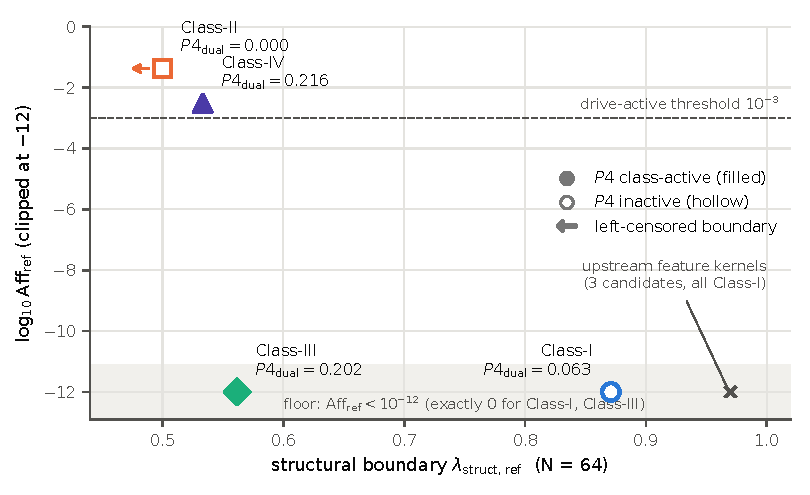
\includegraphics[width=0.8\textwidth]{figures/observable_map.pdf}
\caption{The four representatives on a common observable map ($N=64$, manual lens). Horizontal: structural boundary. Vertical: affinity at the boundary (log scale; the shaded floor holds readings below $10^{-12}$, which for Class-I and Class-III are exact zeros). Filled markers have staging on, hollow markers have it off. The Class-II boundary is left-censored (arrow). Grey crosses: three kernels built from upstream compiled features, all classified Class-I.}
\label{fig:four-class-observable-map}
\end{figure}

Table~\ref{tab:four-class-observable-coordinates} and Figure~\ref{fig:four-class-observable-map} show the result. The drive axis splits the classes into two pairs: Class-II and Class-IV sit above the drive-on threshold, and Class-I and Class-III sit at exact zero. The staging coordinate splits them the other way: Class-III and Class-IV have $P4_{\mathrm{dual}}\approx0.2$, while Class-I and Class-II have $0.063$ and $0$. Neither coordinate separates all four classes on its own, but together they do. The structural boundary does not separate the classes, but it records where each birth happens. Class-I forms structure latest ($\lambda\approx0.87$). The displayed boundaries of the other three lie between $0.50$ and $0.56$, but for Class-II the value $0.50$ is only an upper bound.

At $N=64$ the Class-II boundary is left-censored. Both structural thresholds are already met at the first grid point, $\lambda=0.5$, so the boundary is known only to lie at or below $0.5$. Its true position on the horizontal axis could be well to the left of the plotted point. This affects where Class-II sits along that axis but not its class. The affinity reading is taken at the censored boundary, $\lambda=0.5$, and is $4.23\times10^{-2}$, far above the drive-on threshold. The affinity curve decreases with $\lambda$ (Figure~\ref{fig:drive-curves}), so any boundary further to the left would give a larger reading.

This map is the main synthetic result of the paper. Its value is that it is built directly from the observables that define the classes. It does not depend on exponent fits, which remain unreliable here (Appendix~\ref{app:negative-results}). It is a map of four representative systems, not a phase diagram of the parameter space.

\subsection{Upstream feature kernels}

To test whether the observables can be computed on systems from outside our synthetic families, we built kernels from a vendored copy of the upstream Six-Birds closure library. Three symbolic instances (\texttt{tau\_conflict}, \texttt{audit\_sector}, and \texttt{audit\_partition\_loop}) were compiled by the library's own compiler into substrates with 22, 50, and 54 states. From each compiled substrate we constructed a kernel: a row-normalized Gram matrix of the compiled features with a boost within each sector, mixed with an artificial preference-gradient term. This is therefore a kernel derived from upstream features, not the upstream system's native dynamics.

All three kernels run through the same pipeline and receive the label Class-I. They have structural boundaries near $\lambda\approx0.97$, affinities of order $10^{-23}$ (drive off), and $P4_{\mathrm{dual}}\approx0.014$ (staging off, though a weak $P4$-like signal is present). They appear as the grey crosses in Figure~\ref{fig:four-class-observable-map}. The result shows that the map can be applied to kernels from another codebase. It does not show that the upstream system realizes the other three classes, and the ``high'' confidence reported by the bridge is a heuristic, not a statistical statement.

\subsection{Capacity and depth after birth}

We also measured post-birth proxies for each representative: the remaining closure-strength headroom $1-\lambda_{\mathrm{struct,ref}}$, how long (in $\tau$) the structural targets survive, the area under the objecthood curve across $\tau$, and a combined capacity--depth index. Under the packaging control these proxies are not independent of the birth location. At $\lambda=1$ the dynamics is the idempotent kernel $QU$, so for every positive $\tau$ we have $\mathrm{CE}=0$ and $M_{\mathrm{obj}}=1$, and with the uniform two-block lift also $\mathrm{Aff}=0$. Depth survival and objecthood area therefore saturate at the same values for all four classes, and the combined index reduces algebraically to $(1-\lambda_{\mathrm{birth}})\cdot\tau_{\max}$, where $\tau_{\max}=8$ is the largest sampled timescale and $\lambda_{\mathrm{birth}}$ is the structural boundary measured by the capacity campaign. In other words, the capacity index is a rescaled copy of a structural boundary proxy. That proxy is measured on campaign-specific grids: the scaling-campaign grids for Class-I and Class-II and the full-campaign grids for Class-III and Class-IV. For Class-II these differ from the map grid. There the grid starts at $\lambda=0.4$, and the Class-II capacity reference ($0.4$ at $N=64$) is again left-censored. Consistent with this, it does not line up cleanly with either the drive axis or the staging axis. We report it as a description of what happens after birth, not as a classifier, and we draw no further conclusion from it.
